\section{Results}
\label{sec:results}

In this section we present the outcome of our implementation.
\todoRevise{update results with correct values}

%% --------------------------------------------

\subsection{Kernel Model}
\label{subsec:kernmodel}

For constructing a model to register the data, we ended up using the following: 
$$ k(5, 20) + k(10, 50) + k(100, 200) $$
where $k(s, \sigma)$ is a diagonal kernel of Gaussian kernels with variance $\sigma$ scaled with $s$. 
\autoref{fig:kernel_model} shows its mean in orange and some samples of its variability in white.

\begin{figure}
	\centering
  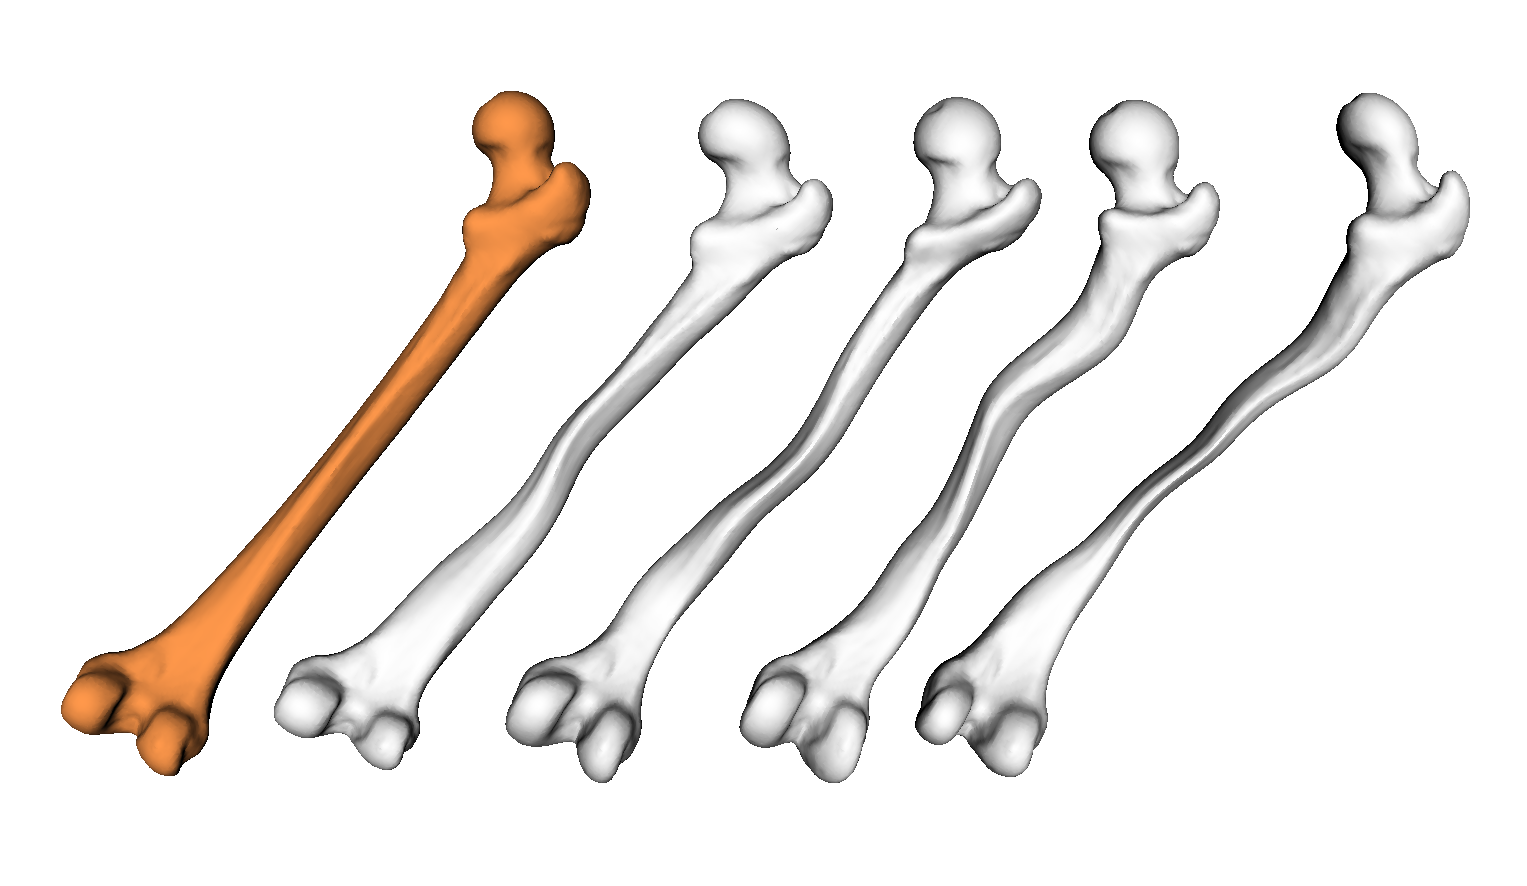
\includegraphics[width=\columnwidth]{./Figures/kernel_model_samples}
  \caption{
    The mean of our kernel model shown in orange. 
    Alongside are shown some random samples of the model.}
  \label{fig:kernel_model}
\end{figure}

%% --------------------------------------------

\subsection{Registrations}
\label{subsec:registrresults}
While in the end we are only interested in the distance between our reconstruction and the ground truth, we can also use the distance metrics as an indication of how closely our kernel model fits the training data. 
Hopefully, a better representation of our training data also leads to a better reconstruction of the partial bones. 

The mean and standard deviation of the average and the Hausdorff distance are provided in \autoref{tbl:registration_distance}.
In \autoref{fig:registration_fit} you can see an example of the kernel model fitted to the training data.

\begin{table}
\centering
\caption{Distances from fitted model to training data}
\label{tbl:registration_distance}
\begin{tabular}{lrr}
\toprule
\textbf{Bones} &
Average Distance &
Hausdorff Distance \\
\midrule
Mean& 0.63 & 11.05 \\
Standard Deviation& 0.28 & 15.45 \\
\bottomrule
\end{tabular}
\end{table}

\begin{figure}
	\centering
  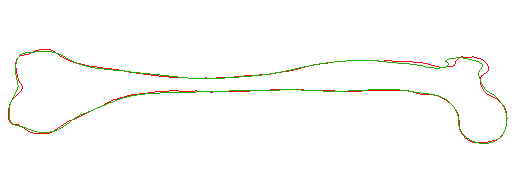
\includegraphics[scale=0.7]{./Figures/registration_fit}
  \caption{Example registration of the model to a bone from the training data}
  \label{fig:registration_fit}
\end{figure}

%% --------------------------------------------

\subsection{Trained Model}
\label{subsec:trainedmodel}
\autoref{fig:trained_model} shows the trained model we generated by interpolating the deformation fields of our reference to the reconstructions.

\begin{figure}
	\centering
  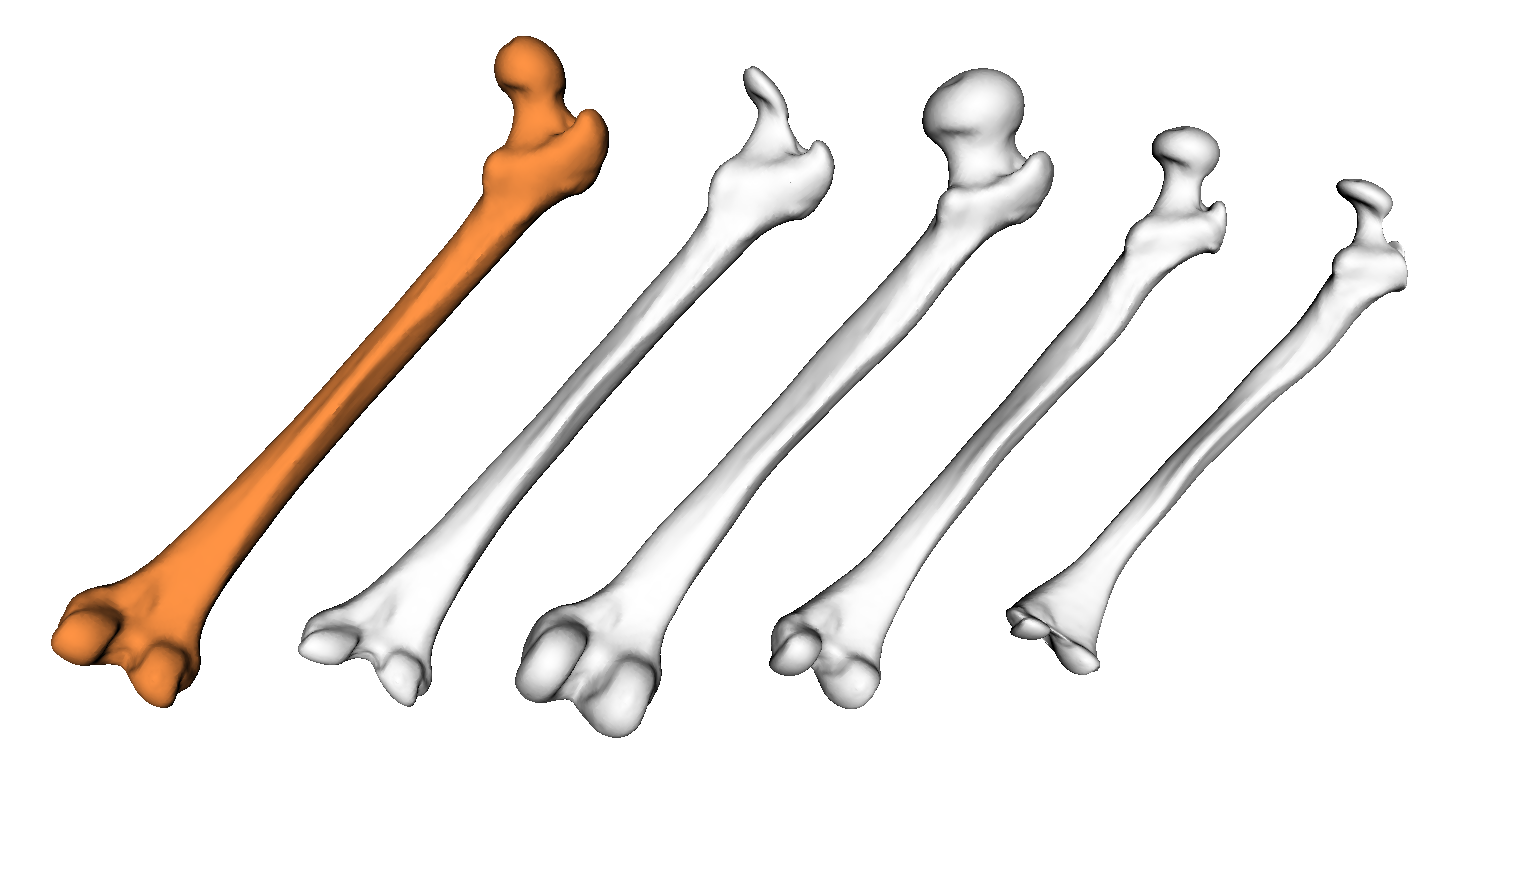
\includegraphics[width=\columnwidth]{./Figures/interpolated_model_samples}
  \caption{
    The mean of our trained model shown in orange.
    Alongside are shown some random samples of the model.}
  \label{fig:trained_model}
\end{figure}

%% --------------------------------------------

\subsection{Reconstruction of Partial Femurs}
\label{subsec:reconresults}
For the evaluation of the reconstruction of partial bones, we are interested in closely modelling the actual bone.
In other words, we want our reconstruction and the ground truth data (not given to us) to be as close as possible. 
This will be evaluated using both the average distance and the Hausdorff, both of which should ideally be as small as possible.

\autoref{fig:reconstructed} shows all ten partial femurs aligned to our reconstruction.
The average distance and Hausdorff distance scores of the missing part can be found in \autoref{tbl:reconstructed_distance}.
Only the missing part of the femurs is considered in these error measures.

\begin{figure*}
	\centering
  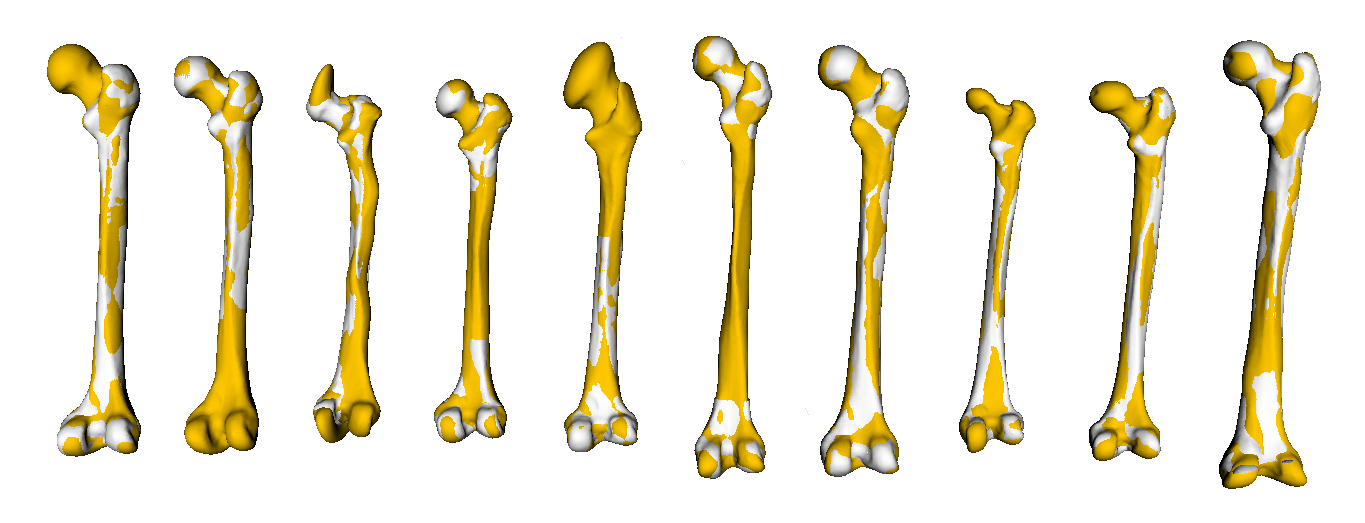
\includegraphics[width=0.82\textwidth]{./Figures/reconstruction_summary}
  \caption{All partial femurs displayed in white, aligned with our reconstruction, displayed in yellow.}
  \label{fig:reconstructed}
\end{figure*}

\begin{table}
\centering
\caption{Distances from reconstructed bone to ground truth.}
\label{tbl:reconstructed_distance}
\begin{tabular}{lrr}
\toprule
\textbf{Bones} &
Average Distance &
Hausdorff Distance \\
\midrule
Bone 1& 2.44 & 5.40 \\
Bone 2& 3.23 & 10.28 \\
Bone 3& 3.64 & 14.46 \\
Bone 4& 1.92 & 9.46 \\
Bone 5& 5.16 & 40.97 \\
Bone 6& 3.65 & 21.59 \\
Bone 7& 2.65 & 11.91 \\
Bone 8& 3.71 & 12.27 \\
Bone 9& 2.14 & 5.42 \\
Bone 10& 7.46 & 24.89 \\
\midrule
Average& 3.6 & 15.66 \\
Standard Deviation& 1.57 & 10.32 \\
\bottomrule
\end{tabular}
\end{table}